\documentclass{IEEEtran}
\usepackage{graphicx} %for PDFLaTeX (pdf, png)
\usepackage{graphics} %for LaTeX (eps, tif)
\usepackage{algorithm}
\usepackage{algorithmic}
\usepackage{array}% http://ctan.org/pkg/array
\usepackage{tabularx}
\usepackage{cite}
\usepackage{caption}
\usepackage{subcaption}
\begin{document}
\title{COSC 4P80: Assignment 2 \\ Experimentation and Investigation of Self-Organizing Maps} %specify the title

\author{\IEEEauthorblockN{Michael Young}\\		%specify the author(s)
\IEEEauthorblockA{Brock University\\
St. Catharines, Ontario\\
Email: my08tu@brocku.ca}}

\maketitle					%tell LaTeX to render the title

\begin{abstract}
Now that we're in the information age, data mining is becoming more and more popular. Self-Organising Maps turns out to be a great tool in manipulating large dimensional data and projected it in a lower dimension that makes it easier to understand. By using various forms of clustering techniques, we are able to analysis large sets of data in hopes that some hidden attribute of the data might be recognized.  The number of applications for a Self-Organizing map is practically endless and in this paper we will discuss the basic problems with clustering as well as see an application for clustering of images. Naturally, will this algorithm their are various parameters that can be altered to obtain various results in the final outcome. This paper will explore some of these parameters and investigate their behaviour and effect on the final resutls.

Key Terms - Self-Organizing map, clustering, image analysis.   
\end{abstract}

%define the rest of your sections
\section{Introduction}{
	The main focus of this paper is to investigate the behaviour of clustering using Self-Organising Feature Maps (SOMs) and how changes in the parameters effect the changes in map clusters. There are numerous ways to cluster information, but for the purpose of the assignment the main focus will be on  Self-Organizing Maps and how it can be used for image clustering. There are a variety of parameters involved in Self-Organising Map and this paper will also investigate altering some of these parameters and determining the effect  it has on the performance of the Self-Organizing Map. Some of the parameters of a SOM include Neighbourhood size and shape, learning rate, exponential decay constant and map dimensions.
}

\section{Problem}
The objective of this assignment is to experiment with Kohonen Self Organizing Maps in order to determine their behaviour when using different parameters, equations, and sample types.

The problem is broken down into two main parts: Colour Organization and Image Clustering.

\subsection{Problem 1. Colour Organization}
The first problem of the paper involves color organization. This can be viewed as a toy problem or a basic example to demonstrate the behaviour of clustering, and more specifically, how SOMs themselves, can be used to perform clustering. This is done by creating a randomly generated image, each pixel has a random RGB value and feeding random samples from this image as training examples for the network. There is further information on this problem in the Data and Samples section.


\subsection{Problem 2. Image Clustering}
The second problem involves image clustering. The goal of image clustering is to provide the network with enough training examples so that while the network is training, the images are placed in similar groups based on differing color features. Images are partitioned and information regarding the color of each pixel are encoded in a vector that will be used for training.

The purpose of grouping similar images is in hope that when the network is presented with a new image it hasn't seen before, it can properly classify it as the same type as of other images in a similar clusters. In addition to being able to classify new images, the goal of the SOM is to organize 
More information on Colour Organization and Image Clustering problems can be found in the Data and Samples section.


\section{Neural Networks}
Artificial Neural Networks is a computational model that is inspired by biological neural networks, for example, the
human brain. By connecting a certain number of neurons together to make a layer, then connecting these layers together
through a series of connections each with their own weight, we are able to make a crude approximation of a biological
neural network.

 Using this biological inspiration, it's possible to construct multiple types of networks that have different functionalities. Of the most common is Feed Forward Neural Network. A Feed Forward Neural Network is trained using a supervised training method where the outcome of the training examples are known before hand. The output of the network is then compared to the expected output and the network is modified accordingly to help converge to these expected values.
 
 Sometimes the information of the expected output is not always known in a data set. This is where we have to switch to a form of unsupervised learning. In the next section we will talk more about unsupervised learning with neural networks.

\subsection{Self-Organizing Maps}
Self-Organizing maps(also known as Kohonen Maps, Kohonen Self-Organizing Maps or simply SOMs) are a specific type of neural network. Originally developed by Tuevo Kohonen in 1982, SOMs are based on the associative neural properties of the brain and inspired by the grouping structure of neurological connections. The way SOMs learn and are trained in specific applications can be viewed as a form of competitive learning, as well as an added co-operative feature. This represents a form of unsupervised learning, where the outcome of training examples is not known.\cite{thesom}

	Another property of SOMs is their ability to transform high dimensional data into a lower dimension while still preserving the data's topology. This gives us the ability to observe possibly interesting features in data that otherwise might not be clear.\cite{somvismethods}
	
	There are a variety of applications for SOM's, more can be found in Kohonen's Engineering Applications of the Self-Organizing Map \cite{eng_app_of_soms}. An interesting and widely used example can be found on ai-junkie.com\cite{aijunkie}. In this example the quality of life was measured for a variety of countries and were fed through the SOM. These factors can include country health, nutrition, educational services etc. The outcome is a map based on the different qualities of life that were measured. As shown in figure \ref{fig:qolmap1}, countries with similar quality of life have been clustered together into their own separate groups. It's clear from this picture that the quality of life in Belgium (Orange cluster) is drastically different that of Kenya (light blue).
	
	With this map information, it's possible to project this information differently to get a more in depth understanding of the map and how it relates to the quality of life. Referring to figure \ref{fig:qolmap2} each country has been coloured according to it's cluster value of the map. This picture now shows us even more information such as where exactly on the globe that the quality of life is similar or differs.

\begin{figure}[!htbp]
\centering
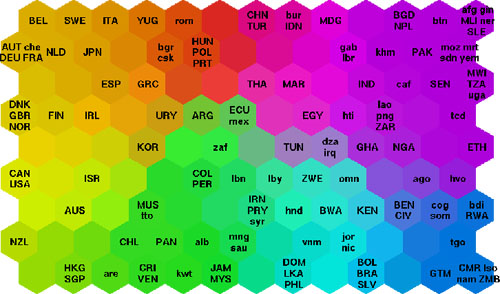
\includegraphics[scale=0.45]{./images/quality_of_life_map1.jpg}
	\caption{Quality of Life Image Map - Countries with similar quality of life values are clustered together.}
\label{fig:qolmap1} 
\end{figure}	

\begin{figure}[!htbp]
\centering
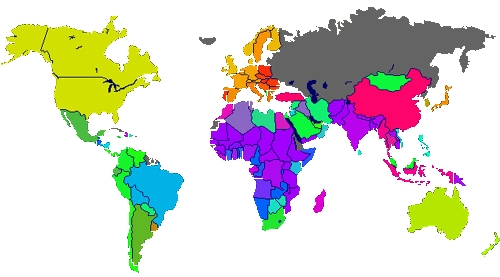
\includegraphics[scale=0.45]{./images/quality_of_life_map2.jpg}
	\caption{Quality of Life Image Map - The colour values from \ref{fig:qolmap1} are displayed on the world map to get a better understanding of the proximity of countries and their corresponding quality of life values.}
\label{fig:qolmap2} 
\end{figure}	
	
		This is just one example of how Self Organising Maps can be used to represent multi-dimensional data into a lower dimensional space. Naturally, this makes understanding the problem and data interpretation much easier for humans.

 
\subsection{Structure}
The structure of the SOM network is quite different from a Feed-Forward Neural Network. The SOM consists of an input layer connected to a 2-Dimensional lattice of neurons called the Kohonen Layer. Each neuron in the layer is connected to each neuron in the lattice. The input layer is similar to that of an input layer in a feed-forward network, where the number of neurons in the layer is equal the dimension of the sample input vector. Each neuron in the Kohonen layer contains a weight vector whose dimension is equal to the of the input vector. The topology of the network can be seen in figure \ref{fig:somstructure}\cite{ascalablesomalg}.


\begin{figure}[!htbp]
\centering
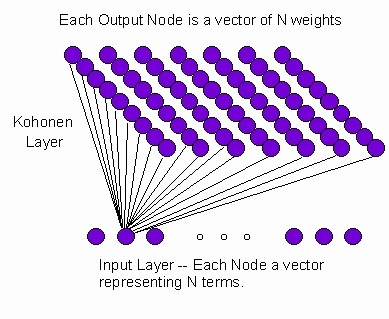
\includegraphics[scale=0.50]{./images/som_structure.jpg}
	\caption{Kohonen SOM Topology - An input vector is connected to a lattice of neurons each with its own weight vector.}
\label{fig:somstructure} 
\end{figure}

\subsection{Algorithm}
The algorithm for SOMs is rather straight forward. Although it's difficult to express the algorithm explicitly in mathematical theorems, it's still possible to achieve an intellectual understanding of the process and outcome of a Self Organizing Map. \cite{thesom}

\begin{algorithm}[!htbp] 
\caption{Self-Organizing Map}
\begin{algorithmic}
\REQUIRE {Initialize the weights in the network}
\WHILE{time $<$ $t_{max}$ and convergence has not be reached}
\STATE Choose random sample vector from data
\STATE Find Best Matching Unit
\STATE Calculate neighbourhood radius of BMU
\STATE Adjust weights accordingly in neighbourhood
\ENDWHILE
\end{algorithmic}
\end{algorithm}

The algorithm can be read as follows. While the clusters are still converging, grab a random sample vector from the data set and pass it through the network. The network then finds the Best Matching Unit(BMU) neuron to the sample vector and updates the weight values of this neuron as well as all the neurons in its neighbourhood by a specified value. This process is repeated until a specified number of iterations or the clusters have converged.

\subsection{Finding the Best Matching Unit}
The Best Matching Unit is the neuron with a weight vector that most closely resembles a given sample vector. Finding the BMU can be considered as a competitive learning technique in which each neuron has a chance to win but only the best is selected. The BMU can be found using a variety of techniques \cite{thesom}. The most popular approach is calculating the distance between the given sample vector and the BMU weight vector. One of the most common distance measures is Euclidean distance, which measures the squared distance between two vectors. Given two vectors, $v_{1} = [x_{1}....x_{n}]$ and  $v_{2} = [y_{1}....y_{n}]$ where n is the number of elements in the vector, then the distance between the two is measured as:

\begin{equation}
distance = \sqrt{(x_{1}-y_{1})^2 + ... + (x_{n}-y_{n})^2}
\end{equation}

The lower the distance, the closer the two vectors are to one another. If we want to find the BMU, all we do is search the network for the neuron that has a weight vector which has the least amount of distance to the given sample vector.

\subsection{Neighbourhood Update}
	The neighbourhood of a given neuron constitutes as an abstract area around the unit in which changes in that neuron will effect other neurons within that area. Once the BMU is found, it's neighbourhood is calculated based on some decay function. It can decay linearly, however it's more common to use an exponential decay function similar to equation \ref{expeq}. $\sigma_{0}$ represents the initial neighbourhood radius. A new radius is calculated basic on the decay function with respect to time $t$ and a decay constant $\lambda$. This process of updating the weights in a specific neighbourhood can be viewed as a form of co-operative learning, where the neurons work together to more similar to the BMU. \cite{thesom}  

\begin{equation}
\sigma(t) = \sigma_{0} e^{\frac{-t}{\lambda}}
\label{expeq}
\end{equation}

	The initial choice in the radius of the neighbourhood can alter the outcome of the SOM drastically. The radius has to be large enough to ensure that enough neurons in the lattice are getting a chance to fire. If the radius is too small, a sporadic behaviour appears in the map and the direction of ordering for the cluster will change discontinuously. \cite{thesom}  There is a more in depth explanation in the Analysis section on the effects of the initial neighbourhood radius size.

\subsection{Learning Rule}
	The learning rate for the network work represents how big of factor to apply to the weight update equation when it comes time to adjust a neuron's vector. The learning rate can vary from values ranging from 0.0 ... 0.9. Initially the factor $\alpha_{0}$ should be a large value, typically somewhere around 0.7-0.9. Like the neighbourhood radius, this value also decays with respect to time according the the following equation:

\begin{equation}
\alpha(t) = \alpha_{0} e^{-t/{\lambda}}
\end{equation}

Where $\alpha(t)$ represents a new learning rate at the given time $t$. By continuously decaying the learning rate, this allows the network to initially makes large changes in the weights to more quickly isolate clusters, then over time, to help the network converge, the small learning rate will help make the minor changes necessary to get the best characteristics from a cluster.

\subsection{Weight Update}
Once the BMU is found and the neighbourhood radius is calculated, the new learning rate found above is applied to the following weight update equation:

\begin{equation}
W_{i+1} = W_{i} + \alpha(t)(V_{i} - W_{i})
\label{eqn:weightupdate}
\end{equation}

The new weight is found by adding the old weight plus the learning rate multiplied with the difference between the sample vector $V_{i}$ and the weight vector $W_{i}$. By updating the weights in this manor, the weight vectors of the neighbourhood neurons will update accordingly and make their vectors more similar to the sample vector. Repeating these steps over a number of iterations allows the network to properly learn and classify the data set it's been given. 

\section{Data and Samples}
\subsection{Problem 1 - Colour Organization}
The goal of this problem is to present the SOM with randomly coloured pixels and have it classify them in similar groups based on their Red, Green and Blue colour values. An initial image of 200x200 pixels is created as shown in figure \ref{fig:randsample}. The random colors chosen are limited to 8 different colours as shown in table  \ref{tab:colordata}

{\renewcommand{\arraystretch}{2}%
\begin{table}[!htbp]
\caption {Random Colour Values} \small
\centering
\begin{tabular}{|l|l|}
\hline
Colour & (R,G,B) Value\\
\hline
Red & (255,0,0) \\
\hline
Magenta & (255,0,255) \\
\hline
Blue & (0,0,255) \\
\hline
Cyan & (0,255,255) \\
\hline
Green & (0,255,0) \\
\hline
Yellow & (255,255) \\
\hline
Black & (0,0,0) \\
\hline
White & (255,255,255)\\
\hline
\end{tabular}
\label{tab:colordata}
\end{table}
}

\begin{figure}[!htbp]
\centering
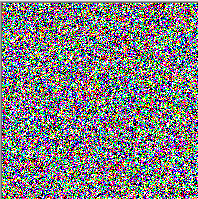
\includegraphics[scale=0.40]{./images/randomsample.png}
	\caption{Random Sample Image - 200x200 pixel colours of image are randomized to get 8 different colours, namely - Red, Magenta, Blue, Cyan, Green, Yellow, Black, White. Each pixel will serve as a data sample.}
\label{fig:randsample} 
\end{figure}

For every iteration of the SOM algorithm, a pixel is randomly chosen from this image. The sample vector is constructed using the RGB values and it's this vector that will be used to find the Best Matching Unit in the network. The objective here is to obtain a classification for each colour based on it's corresponding cluster. An example of the map after training is shown in figure \ref{fig:orgnaizedcolors}. Note how clusters that have similar shade in color, like green, yellow and cyan are positioned closer to one another. As opposed to colours with high contrast like black and white, their positions differ greatly on the map.

\begin{figure}[!htbp]
\centering
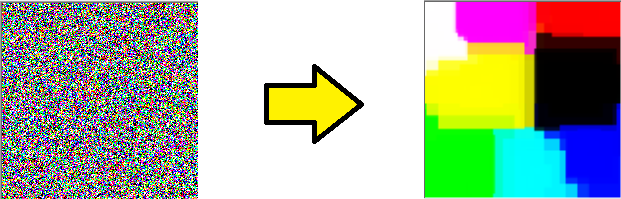
\includegraphics[scale=0.50]{./images/random_to_organization.png}
	\caption{Random to Organized - The random colours of the picture on the left have been fed through the network and the SOM has grouped them accordingly. Clusters sharing a similar colour are closer together than clusters with varying colours.}
\label{fig:orgnaizedcolors} 
\end{figure}

\subsection{Problem 2 - Image Clustering}
Image clustering works similar to the previous problem, however this time our sample vectors are no longer going to be random RGB values. For image clustering, we want to pass through the network whole images in hopes that it can classify a variety of images based on some unique features. For this analysis a group of images was chosen at random. I chose to use characters from the Super Nintendo game Donkey Kong Country. I chose 7 different characters, as shown in figure \ref{fig:picturesamples} from the game and gathered 3 images of each for training data, although just one picture for each character is shown. Note that there are only two images for Krusha, I was unable to find a suitable third picture. 

\begin{figure}[!htbp]
\centering
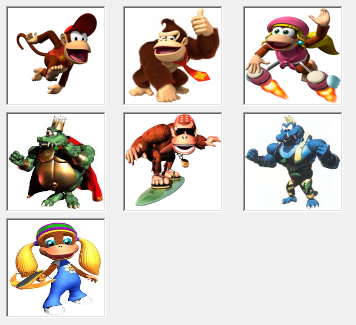
\includegraphics[scale=0.50]{./images/picture_samples.png}
	\caption{Sample Images - Sample images used in training. Starting from the top left going right - Diddy Kong, Donkey Kong, Dixie Kong, King K. Rool, Funky Kong, Krusha, Tiny Kong. Note that there are a total of 3 images for each character(excluding Krusha) that are actually used in training.}
\label{fig:picturesamples} 
\end{figure}

Originally the goal was to have the SOM cluster members of the Kong family, however it was quickly realized that the image quality of each was not significant enough to have the SOM produce a clear cluster distinction. The addition of K. Rool and Krusha allowed the SOM to better organize the pictures based on their overall appearance or any hidden data that might be hiding in the higher dimensions.

 The sample vector is constructed differently that the previous RGB vector. A vector $v_{1}$ is constructed that has the form: 

 
\begin{equation}
v_{1} = [\mu(RGB),\sigma(RGB),\mu(R),\sigma(R),\mu(G),\sigma(G),\mu(B),\sigma(B)]
\end{equation}


Where $\mu$(RGB) and $\sigma$(RGB) is the average and standard deviation values respectively for the Red, Green and Blue values for each pixel over the entire image. The rest of the values are corresponding to the average and standard deviation of each Red, Green and Blue color over the entire image.

In order to create a unique classification for each picture, every picture is partitioned into 9 equals parts as shown in figure \ref{fig:dkpartition}.
 
 
\begin{figure}[!htbp]
\centering
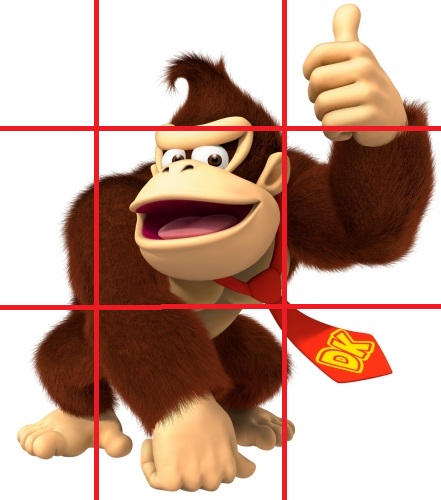
\includegraphics[scale=0.25]{./images/donkeykong_partition.jpg}
	\caption{Example of Image Partition - Every image in the collection is partitioned into 9 equal parts in order to construct a sample vector based on that picture's unique colour qualities.}
\label{fig:dkpartition} 
\end{figure}


Another vector $v_{2}$ in now constructed using each of the partitions information. $v_{2}$ takes the following form:

\begin{equation}
\begin{align}
$v_{2}$ = $v_{1}$ + [\mu(RGB),\sigma(RGB),\mu(R),\sigma(R),\mu(G),\sigma(G),\mu(B),\sigma(B)] \\ \\
$v_{2}$ = [\mu(RGB_{t}),\sigma(RGB_{t}),\mu(R_{t}),\sigma(R_{t}),\mu(G_{t}),\sigma(G_{t}),\mu(B_{t}),\\
		 \sigma(B_{t}), \mu(RGB),\sigma{RGB},\mu(R),\sigma(R),\mu(G),\sigma(G),\mu(B),\sigma(B)]
\end{align}
\end{equation}

Where $|v_{2}| = |v_{1}| + 18 = 8 + 18 = 26$ and where $S_{i}$ respresents the $i^{th}$ subsection of the partitioned image, and $\mu(S_{i})$ and $\sigma(S_{i})$ are the average and standard deviations of the combined Red, Green and Blue values for each section. This new vector $v_{2}$ represents a training vector for the SOM. In total there are 20 sample vectors, each vector representing one of the images respectively.

\section{Analysis}
In order to have a full understanding of Self-Organizing Maps, it's a good idea to have an understanding of the parameters and the effects they have on the network should they be changed. An analysis was done on the neighbourhood size to show the effects of altering the initial radius size. Analysis was also done on the learning rate, and how changes to the initial learning rate values can effect the map. 

Analysis was done using a map size of 200 neurons by 200 neurons and a decay constant of $\lambda = 15.0$. The algorithm ran for a total of 250 iterations. From observation evidence the colour organization seems to converge around that mark, any more iterations and the SOM would be over-fed. 

{\renewcommand{\arraystretch}{2}%
\begin{table}[!htbp]
\caption {Learning Rate Values} \small
\centering
\begin{tabular}{|c|c|}
\hline
$\alpha$\\
\hline
0.9  \\
0.7  \\
0.5   \\
0.2  \\
\hline
\end{tabular}
\label{tab:learningratevalues}
\end{table}
}

{\renewcommand{\arraystretch}{2}%
\begin{table}[!htbp]
\caption {Neighbourhood Radius} \small
\centering
\begin{tabular}{|c|c|}
\hline
$\sigma$\\
\hline
200  \\
100  \\
50   \\
20  \\
\hline
\end{tabular}
\label{tab:neighbourhoodvalues}
\end{table}
}

\subsection{Validity Measures}
Since clustering is a unsupervised training process, the evaluation of the Self-Organizing Map after training is crucial in determining the validity of clusters. There are several clustering validity measures, however we will focus on the Dunn validity measure \cite{clustervaliditymeasurement} . Introduced by Dunn \cite{dunnval}, the Dunn index definition is as follows:

\begin{equation}
D = \min_{i=1..n_{c}} \left\lbrace \min_{j=i+1..n{c}}\left\lbrace\frac{d(c_{i},c_{j}}{\max_{k=1..n_{c}diam(c_{k})}}\right\rbrace \right\rbrace
\end{equation}
\begin{equation}
d(c_{i},c_{j}) = \min_{x c_{i},y c_{j}} \left\lbrace d(x,y) \right\rbrace 
diam(c_{i}) = \max_{x,y  c_{i}} \left\lbrace d(x,y)\right\rbrace
\end{equation}


Where d is the number of dimensions, d(x,y) is the distance between two data elements, $c_{i}$ is a given $i^{th}$ cluster and $n_{c}$ is the number of clusters.


\section{Results} 

\subsection{Neighbourhood Radius Analysis}


\begin{figure}[!htbp]
\centering
\begin{tabular}{cc}
\begin{minipage}{100pt}
\centering
\frame{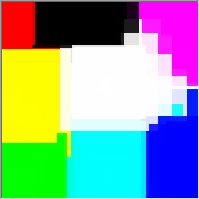
\includegraphics[scale=0.50]{./images/results/1_NR_200.jpg}}
\caption{$\sigma=200$}
\label{fig:1}
\end{minipage}
&
\begin{minipage}{100pt}
\centering
\frame{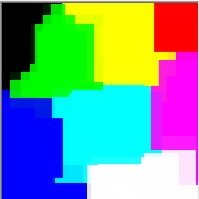
\includegraphics[scale=0.50]{./images/results/2_NR_100.jpg}}
\caption{$\sigma=100$}
\label{fig:2}
\end{minipage}
\\
\begin{minipage}{100pt}
\centering
\frame{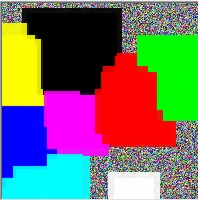
\includegraphics[scale=0.50]{./images/results/3_NR_50.jpg}}
\caption{$\sigma=50$}
\label{fig:2}
\end{minipage}
&
\begin{minipage}{100pt}
\centering
\frame{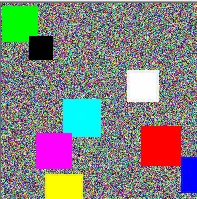
\includegraphics[scale=0.50]{./images/results/4_NR_20.jpg}}
\caption{$\sigma=20$}
\label{fig:2}
\end{minipage}
\end{tabular}
\caption{Neighbourhood Radius Analysis}
\end{figure} 


It's quite clear by looking at the final clusters that having a neighbourhood radius size of $\sigma = 50$ and $\sigma = 20$ are not optimal values. With such a small radius compared to the size of the map, not all neurons get a chance to fire, as shown by the random pixel values in map representing the initially random weights. The neurons that are not fired are considered to be "dead neurons" because  if they never get a chance to fire in the first initial runs, then it's very unlikely that they will ever get a chance and will most likely be a waste of space. As opposed to a large radius size, where the majority of the network gets a chance to fire in the first few iterations. This clearly leads to a more diverse and tightly knit group of clusters. 

\subsection{Learning Rate Analysis}

\begin{figure}[!htbp]
\centering
\begin{tabular}{cc}
\begin{minipage}{100pt}
\centering
\frame{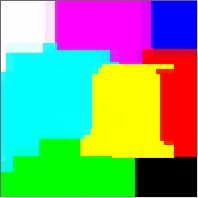
\includegraphics[scale=0.50]{./images/results/1_LR_90.jpg}}
\caption{$\alpha=0.90$}
\label{fig:1}
\end{minipage}
&
\begin{minipage}{100pt}
\centering
\frame{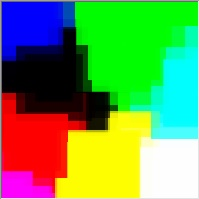
\includegraphics[scale=0.50]{./images/results/2_LR_70.jpg}}
\caption{$\alpha=0.70$}
\label{fig:2}
\end{minipage}
\\
\begin{minipage}{100pt}
\centering
\frame{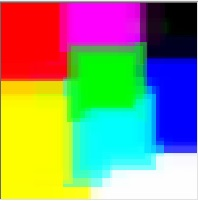
\includegraphics[scale=0.50]{./images/results/3_LR_50.jpg}}
\caption{$\alpha=0.50$}
\label{fig:3}
\end{minipage}
&
\begin{minipage}{100pt}
\centering
\frame{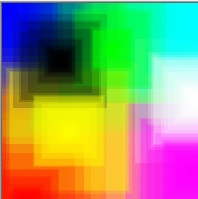
\includegraphics[scale=0.50]{./images/results/4_LR_20.jpg}}
\caption{$\alpha=0.20$}
\label{fig:4}
\end{minipage}
\end{tabular}
\caption{Learning Rate Analysis}
\end{figure} 

The effect of altering the learning rate is rather impressive. It's clear from the images above that modifying the learning rate has an effect on the granularity of the clusters. There isn't two much difference between having an initial learning rate of $\alpha=0.9$ and $\alpha=0.7$, however the change does becomes more noticeable with smaller values. When $\alpha=0.5$ the clusters appear more blurry, not quite as crisp as the previous learning rate. This effect is even more elaborated for $\alpha=0.2$. 
	This would be due to the fact that learning value in the weight update equation \ref{eqn:weightupdate} is a lot smaller that for other values of $\alpha$. This implies there will be less of a change in the weight vector for every neuron in the BMU neighbourhood. In this example this means there will be less change in the color in the neighbourhood and this is reflect in the fuzziness of each cluster. They haven't had a chance to fully learn their own clusters so they are partially merging. 

\subsection{Image Clustering}
The analysis for Image Clustering is to determine if the Self-Organizing map is capable of organizing and clustering a set of images. Using the entire collection of images shown in figure \ref{fig:picturesamples}, a sample collection of 20 vector was constructed and fed through the network. 

Using the following parameters: $\alpha=0.7$, $\sigma=100.0$,$\lambda=15.0$, Map Dimension: 200x200px, 500 Iterations, the following results were produced over a series of runs as shown in figure \ref{results:Imageclustering}

\begin{figure*}
\centering
\begin{tabular}{cc}
\begin{minipage}{200pt}
\centering
\frame{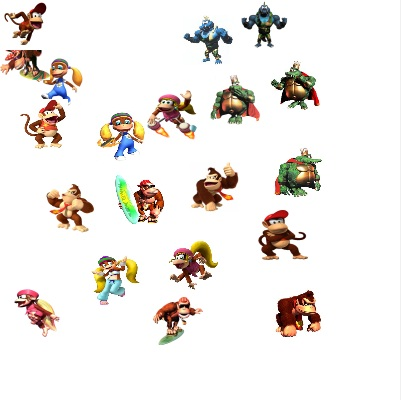
\includegraphics[scale=0.60]{./images/results/cluster_output1.jpg}}
\caption{Result 1}
\label{fig:18}
\end{minipage}
&
\begin{minipage}{200pt}
\centering
\frame{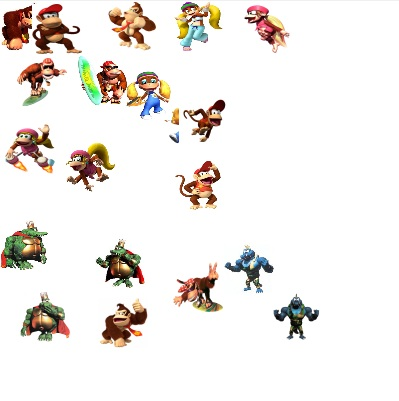
\includegraphics[scale=0.60]{./images/results/cluster_output2.jpg}}
\caption{Result 2}
\label{fig:19}
\end{minipage}
\\
\begin{minipage}{200pt}
\centering
\frame{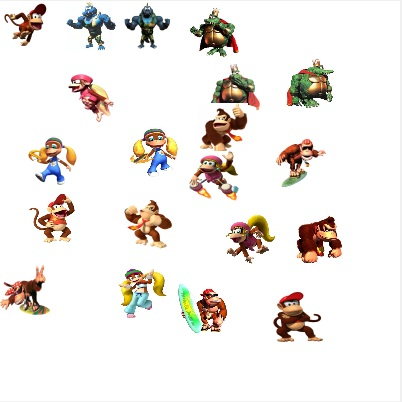
\includegraphics[scale=0.60]{./images/results/cluster_output3.jpg}}
\caption{Result 3}
\label{fig:20}
\end{minipage}
&
\begin{minipage}{200pt}
\centering
\frame{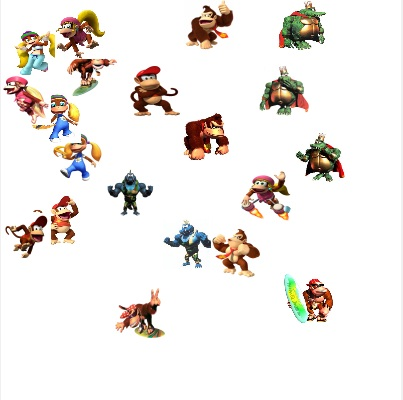
\includegraphics[scale=0.60]{./images/results/cluster_output4.jpg}}
\caption{Result 4}
\label{fig:21}
\end{minipage}
\end{tabular}
\caption{Image Clustering Results - 20 image sample collection. Similar looking images are grouped together. Images with a large difference in appearance are generally farther apart.}
\label{results:Imageclustering}
\end{figure*}

The above samples were made by finding the best matching unit for each picture's sample vector after training and diplsayed their image in their corresponding map position. In all figures it's clear clustering has taken place.
Most noticeable would be the King K. Rool images (Green with a red cape and gold crown).  
The effect of the lighting in each image seems to be effecting the clustering. It's especially noticeable in figure \ref{fig:20}, the images on the bottom-left side have a much greater light effect in their overall image. Where as the images on the top-right area have a much darker appearance. 
Perhaps with a large training set size it would be possible to have the map clustering strictly on each characters personal colour, such that each character as their own cluster. Another possible solution would be to gather more images with similar lighting and graphics resolution.

\section{Conclusion}
The colour organization showed very promising results and displayed a clear indication of the behaviour in varying parameters. By adjusting the initial neighbourhood size, we saw the effects it has on updating nearby neurons and would have to agree with Kohonen \cite{thesom} when an initial size of at least half the map size is sufficient in obtaining optimal clusters.

The image clustering also showed promising results. We saw how the Self-Organizing map breaks apart images to uniquely classify them in the map and how it orders similar pictures based on this classification. It was clear from the results that similar images were indeed being clustered together. However, based on the quality of each image and the overall uniformity, the clustering algorithm still performed well. We saw how some pictures, even though they were the same Donkey Kong Country character, were being  grouped with similar looking pictures that might be due to the brightness or saturation in the picture rather than being grouped with the same character. This might be avoided by choosing a better collection of images or having more training examples of each so the minor differences in each characters will stand out more than their image quality and effects. 


\bibliographystyle{IEEETran}
\bibliography{newbib}

\end{document}
